In this subsection, the performance of the proposed \DAIL{} versus the referenced agents on the high-dimensional task is assessed.
The average cumulative rewards of the evaluated agents are shown in Table \ref{ch:DAIL:tab:Reward_Adroit}.
As expected, the TRPO agent achieved the highest average cumulative reward since it was trained directly on the learner domain.
It is also revealed that \DAIL{} outperformed GAMA-PA, although they were both unable to accomplish the Door-Door task.
In addition, Figures \ref{ch:DAIL:fig:DoorDoor} and \ref{ch:DAIL:fig:HammerHammer} depict the policies learned by TRPO \cite{RL_TRPO}, GAMA-PA \cite{DAIL_Model_DAIL}, and the \DAIL{} agent, from which some interesting behaviors were observed.

\begin{table}[htbp!]
  \centering
  \caption{\added{The performance of the proposed \DAIL{} agent on high-dimensional tasks. These scores represent the cumulative rewards obtained from executing a learned policy in the simulator, averaged over 100 episodes}}
  \label{ch:DAIL:tab:Reward_Adroit}
  % TRPO
% Mean:  2449.0629005253313   Std:  1175.252074139304
% Our
% Mean: -33.50804714371796    Std: 8.870924977649
% GAMA
% Mean:  -65.19344412207603  Std:  0.7695995444977666

% TRPO
% Mean:  17030.245810292417   Std:  4357.225938562724
% Our:
% Mean:  -78.8434             Std:  19.277203
% GAMA:
% Mean:  -252.51961109042168    Std:  4.913654265636941

\begin{tabular}{ccccc}
  \toprule
  \textbf{Task} & \textbf{\DAIL{}}   & \textbf{GAMA-PA} \cite{DAIL_Model_DAIL} & \textbf{TRPO} \cite{RL_TRPO} \\
  \midrule
  Door-Door     & -33.51 $\pm$ 8.87  & -65.19 $\pm$ 0.77                       & 2449.06 $\pm$ 1175.25        \\
  Hammer-Hammer & -78.84 $\pm$ 19.28 & -252.52 $\pm$ 4.91                      & 17030.25 $\pm$ 4357.23       \\
  \bottomrule
\end{tabular}

\end{table}

\begin{landscape}
  \begin{figure}[htbp!]
    \centering
    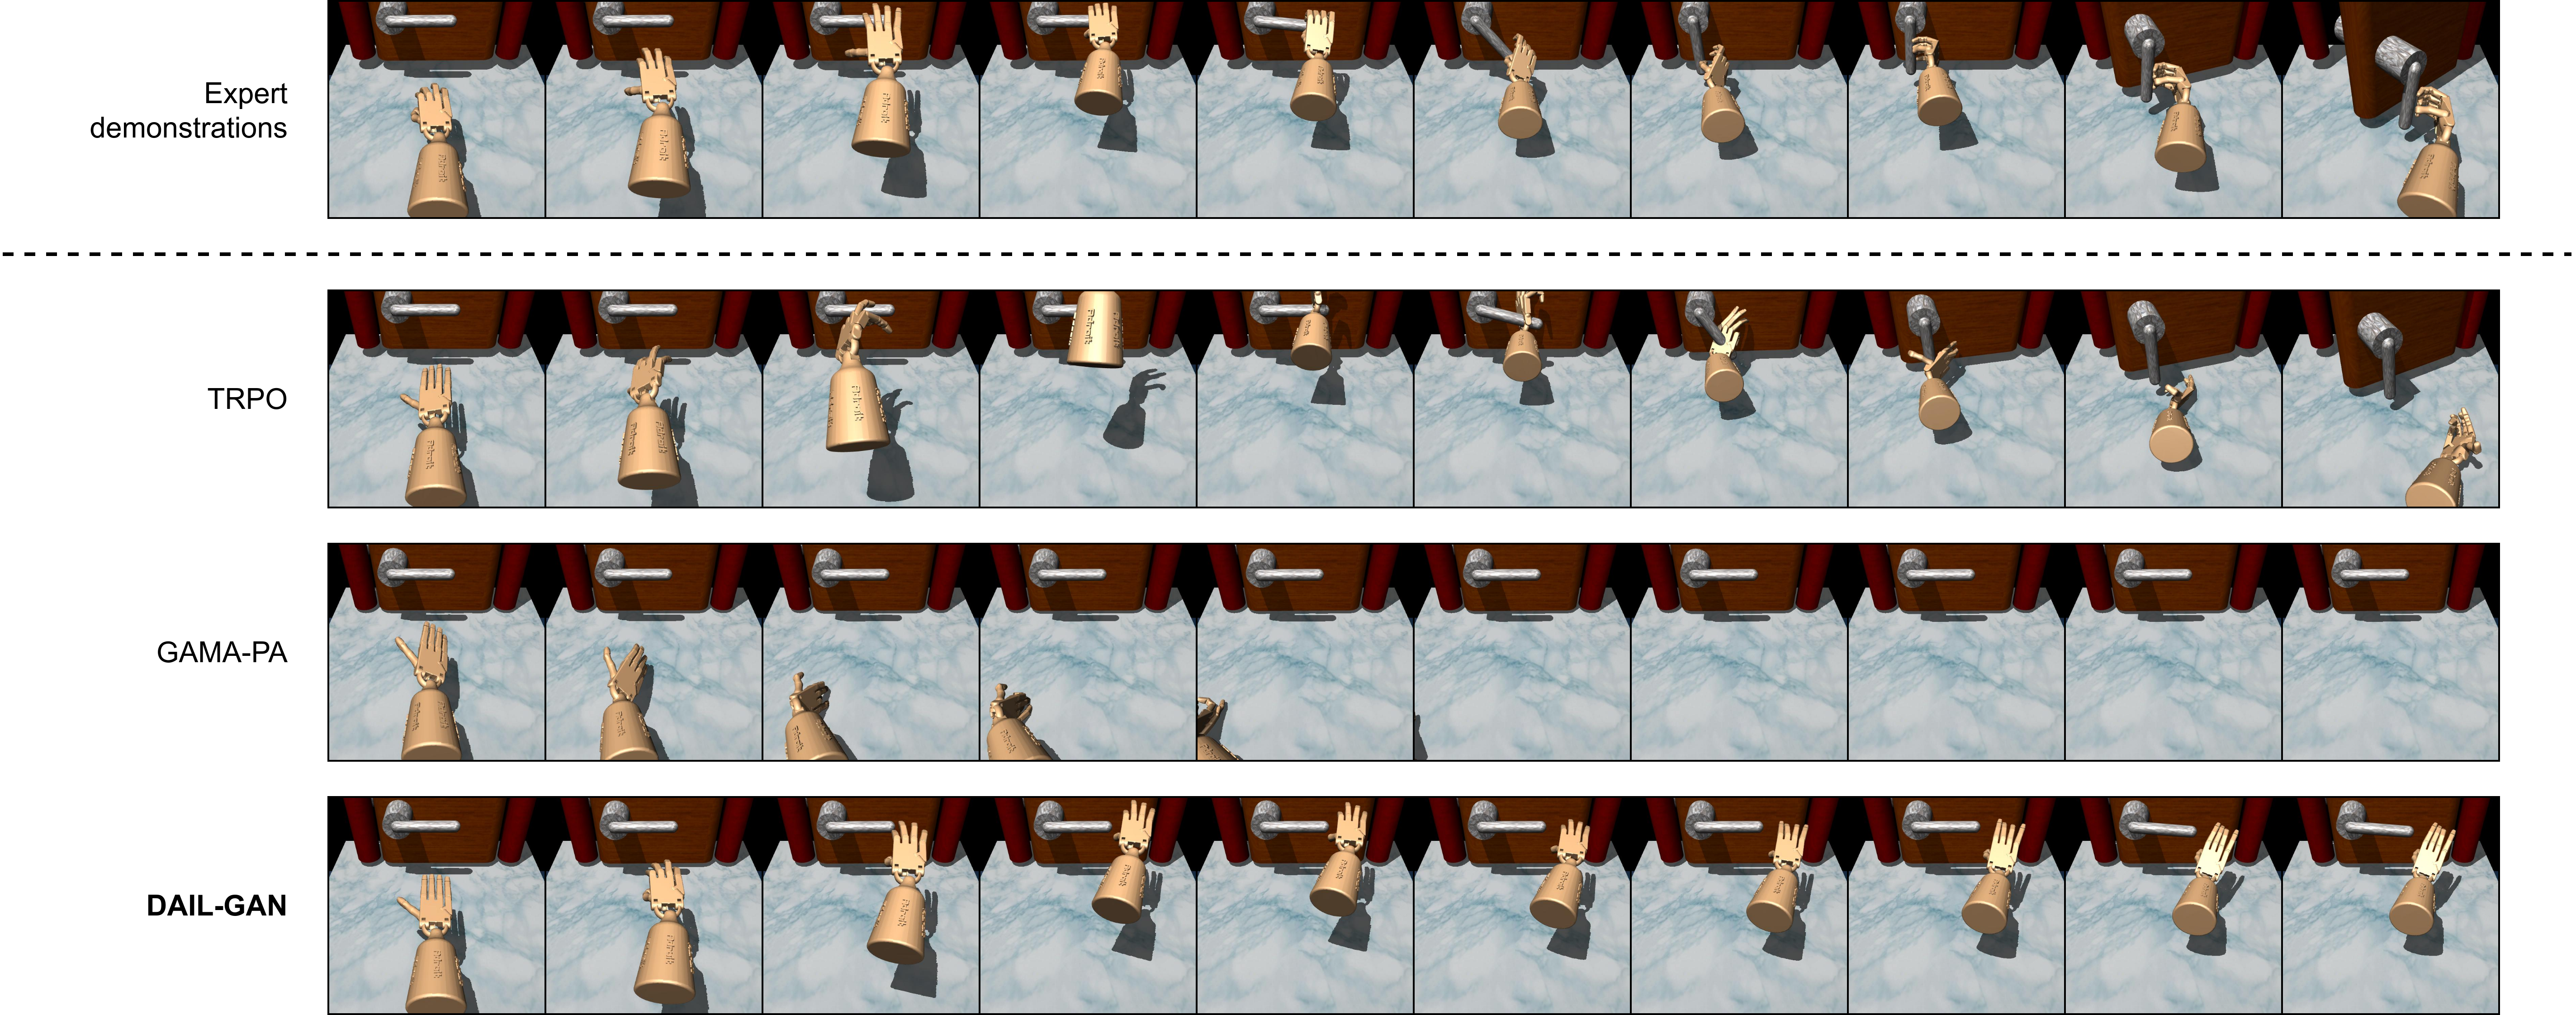
\includegraphics[width=0.7\pdfpageheight]{ \FigsDir/Door-Door.png}
    \caption{Door-Door.}
    \label{ch:DAIL:fig:DoorDoor}
  \end{figure}
\end{landscape}

\begin{landscape}
  \begin{figure}[htbp!]
    \centering
    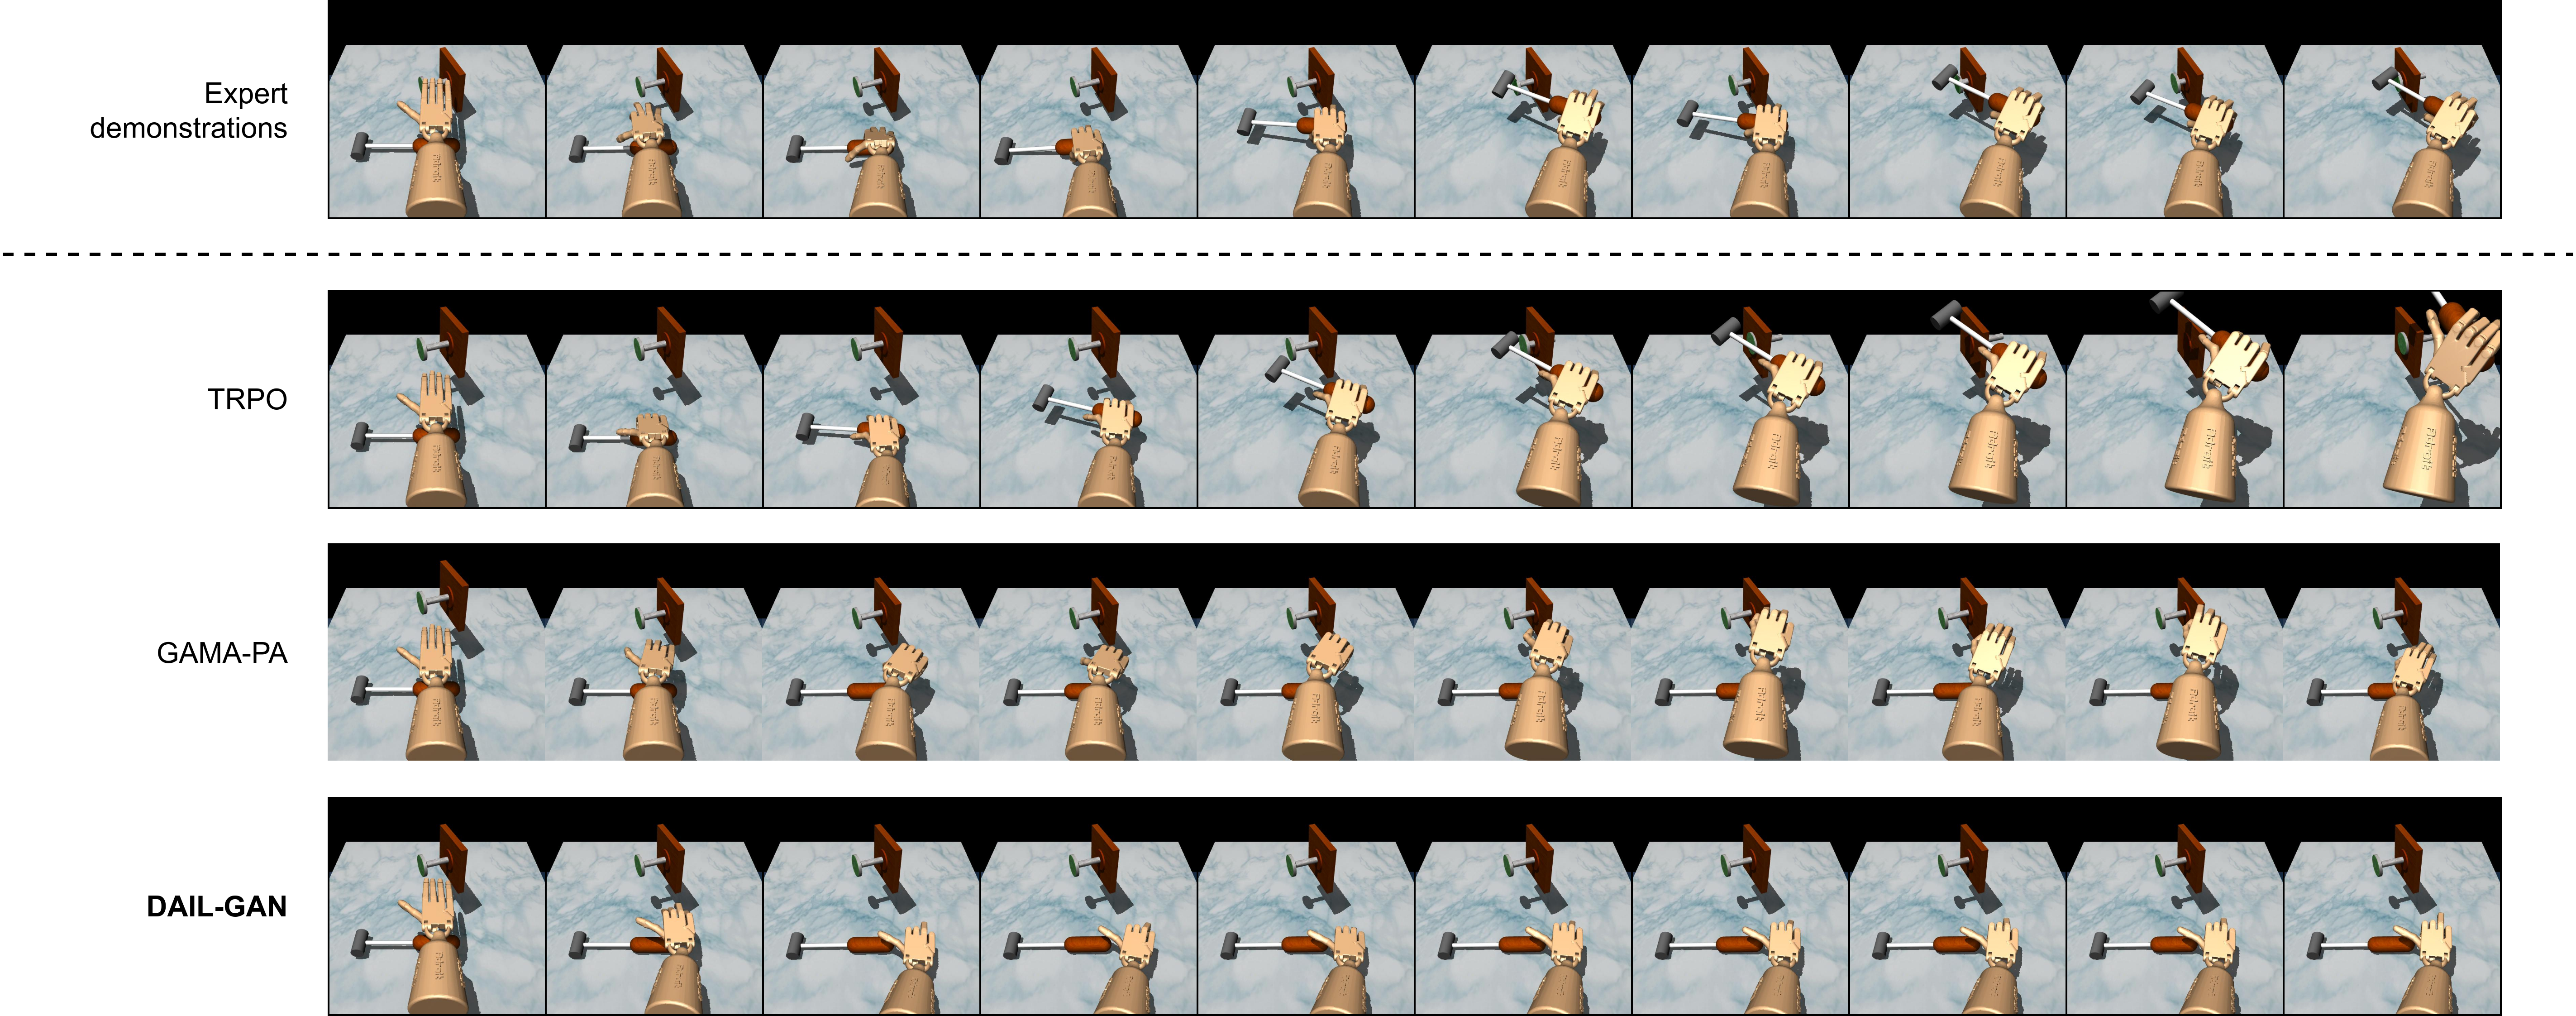
\includegraphics[width=0.7\pdfpageheight]{ \FigsDir/Hammer-Hammer.png}
    \caption{Hammer-Hammer.}
    \label{ch:DAIL:fig:HammerHammer}
  \end{figure}
\end{landscape}

As illustrated in Figure \ref{ch:DAIL:fig:DoorDoor}, the expert behaviors were understandable since their demonstrations were collected from humans: grab the handle, rotate it, then open the door.
In Figure \ref{ch:DAIL:fig:HammerHammer}, the expert behaviors were to pick up and hammer multiple times in order to drive the nail into the board.
While the policy trained with the TRPO could accomplish the task, it produced behaviors that were not human-like, i.e. unnatural use of wrist to rotate the handle.
The main reason behind these unnatural behaviors was that the TRPO depended on a carefully reward shaping and it was challenging to formalize human-like behaviors into a mathematical reward function.
On the other hand, with the use of expert demonstrations, the GAMA-PA and the proposed \DAIL{} were expected to generate human-like behaviors.
Yet, the policy learned by GAMA-PA failed to control the hand properly, as shown in Figures \ref{ch:DAIL:fig:DoorDoor} and \ref{ch:DAIL:fig:HammerHammer}, due to the failure of the adaptation step in high-dimensional task.
Meanwhile, it can be observed from Figures \ref{ch:DAIL:fig:DoorDoor} and \ref{ch:DAIL:fig:HammerHammer} that the policy trained with \DAIL{} could produce more natural and human-like behaviors to move the robot hand closer to the door handle or the hammer.
Unfortunately, \DAIL{} could not rotate the handle or pick up the hammer in order to accomplish the task.
Nevertheless, the human-like behaviors of the trained policies proved that \DAIL{} could effectively extract and imitate expert behaviors from their demonstrations.
